\documentclass[border=4pt]{standalone}

\usepackage{amsmath}
\usepackage{tikz}
\usepackage{mathdots}
\usepackage{yhmath}
\usepackage{cancel}
\usepackage{color}
\usepackage{siunitx}
\usepackage{array}
\usepackage{multirow}
\usepackage{amssymb}
\usepackage{gensymb}
\usepackage{tabularx}
\usepackage{booktabs}
\usetikzlibrary{fadings}
\usetikzlibrary{patterns}


\begin{document}
 



\tikzset{every picture/.style={line width=0.75pt}} %set default line width to 0.75pt        

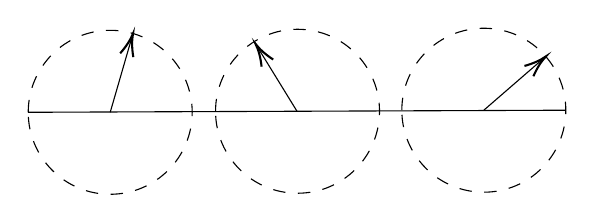
\begin{tikzpicture}[x=0.75pt,y=0.75pt,yscale=-1,xscale=1]
%uncomment if require: \path (0,300); %set diagram left start at 0, and has height of 300

%Straight Lines [id:da7594916287536151] 
\draw    (49,134) -- (308,133) ;


%Shape: Circle [id:dp3595894580281451] 
\draw  [dash pattern={on 4.5pt off 4.5pt}] (49,134) .. controls (49,112.18) and (66.68,94.5) .. (88.5,94.5) .. controls (110.32,94.5) and (128,112.18) .. (128,134) .. controls (128,155.82) and (110.32,173.5) .. (88.5,173.5) .. controls (66.68,173.5) and (49,155.82) .. (49,134) -- cycle ;
%Shape: Circle [id:dp7273196821667289] 
\draw  [dash pattern={on 4.5pt off 4.5pt}] (139.25,133.5) .. controls (139.25,111.68) and (156.93,94) .. (178.75,94) .. controls (200.57,94) and (218.25,111.68) .. (218.25,133.5) .. controls (218.25,155.32) and (200.57,173) .. (178.75,173) .. controls (156.93,173) and (139.25,155.32) .. (139.25,133.5) -- cycle ;
%Shape: Circle [id:dp08540487469939939] 
\draw  [dash pattern={on 4.5pt off 4.5pt}] (229,133) .. controls (229,111.18) and (246.68,93.5) .. (268.5,93.5) .. controls (290.32,93.5) and (308,111.18) .. (308,133) .. controls (308,154.82) and (290.32,172.5) .. (268.5,172.5) .. controls (246.68,172.5) and (229,154.82) .. (229,133) -- cycle ;
%Straight Lines [id:da6412847735417944] 
\draw    (88.5,134) -- (98.94,97.92) ;
\draw [shift={(99.5,96)}, rotate = 466.14] [color={rgb, 255:red, 0; green, 0; blue, 0 }  ][line width=0.75]    (10.93,-3.29) .. controls (6.95,-1.4) and (3.31,-0.3) .. (0,0) .. controls (3.31,0.3) and (6.95,1.4) .. (10.93,3.29)   ;

%Straight Lines [id:da683612424305297] 
\draw    (178.5,133.5) -- (159.55,102.7) ;
\draw [shift={(158.5,101)}, rotate = 418.39] [color={rgb, 255:red, 0; green, 0; blue, 0 }  ][line width=0.75]    (10.93,-3.29) .. controls (6.95,-1.4) and (3.31,-0.3) .. (0,0) .. controls (3.31,0.3) and (6.95,1.4) .. (10.93,3.29)   ;

%Straight Lines [id:da6286834382517008] 
\draw    (268.5,133) -- (296.99,108.31) ;
\draw [shift={(298.5,107)}, rotate = 499.09] [color={rgb, 255:red, 0; green, 0; blue, 0 }  ][line width=0.75]    (10.93,-3.29) .. controls (6.95,-1.4) and (3.31,-0.3) .. (0,0) .. controls (3.31,0.3) and (6.95,1.4) .. (10.93,3.29)   ;





\end{tikzpicture}

\end{document}
